\pagestyle{empty}
\cleardoublepage
\pagestyle{fancy}
\chapter{Direções Futuras}\label{cap4}

Foi feito um estudo nessa área de geração de malhas voltado para a subdivisão de domínios bidimensionais. Já foi dado início ao desenvolvimento de uma técnica de geração de malha baseada num particionamento utilizando \textit{quadtree}.

Este trabalho que estou propondo pode ser dividido basicamente em duas etapas. A primeira consiste em receber a entrada e dividi-la em pedaços que possam ser tratadas como novos domínios. Todos esses pedaços por sua vez possuem a quantidade de carga aproximadamente equivalentes.

Existem vários pesquisadores estudando novas formas de subdividir domínios para geração de malhas tanto tridimensionais como bidimensionais. A técnica proposta utiliza uma \textit{quadtree} para estimar a carga de cada subdomínio que for gerado para se obter um bom balanceamento de carga entre os processadores.

A segunda etapa será a geração da malha em cada um dos novos domínios. Qualquer algoritmo de triangulação dado uma borda como entrada pode ser utilizado, inclusive podem ser empregado algoritmos diferentes nos subdomínios. Além da triangulação, tem que ser feita a junção das diversas malhas geradas em uma só.

Para esse trabalho estou propondo uma técnica de geração de malha por avanço de fronteira por particionamento do domínio em paralelo. O foco da técnica é a subdivisão dos domínios e não a geração da malha. O algoritmo de avanço de fronteira que estou utilizando para gerar malha está em \cite{bib:Miranda99} e \cite{bib:Cavalcante-Neto01}.

\section{Cronograma}
Nesta seção apresento o cronograma de estudo e trabalho para conclusão da dissertação de mestrado.

 \begin{figure}[htbp]
     \begin{center}
     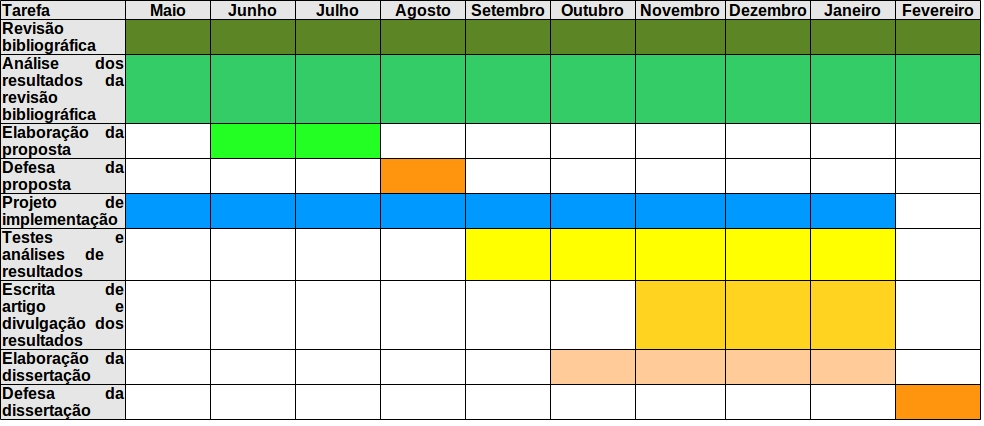
\includegraphics[width=1.1\textwidth]{tabela}
     \label{fig:tabela}
     \end{center}
 \end{figure}